\section{Result II: Blind Rollout Tests Predictor Geometry}
\label{sec:imagine}

The spectral theorem (\cref{sec:nonforget}) preserves the joint-state
spectrum exactly but says nothing about whether useful reduced-state
information survives a long imagined trajectory. This section measures
how much of the target encoder's representation is recoverable after
$k$ blind predictor steps, and compares UWM-JEPA against a
parameter-matched LSTM-JEPA under a single protocol.

\paragraph{Protocol}
Training uses a partially observed CartPole-style spring benchmark with
a JEPA objective (online encoder, EMA target encoder, latent-space
loss, stop-gradient on the target
branch)~\cite{hafner2020dream,hafner2019learning}. All models in this
experiment are trained at horizon $k=5$, so $k=1$ and $k=3$ test
intermediate rollout coherence while $k=10$ and $k=20$ test
extrapolation beyond the trained horizon. At evaluation time we fix a
context $x_{\le t}$, obtain the predicted latent
$\hat z_{t+k} = P_k(E_\theta(x_{\le t}))$, and compare it against the
target latent $z_{t+k}^+ = E_{\xi}(x_{\le t+k})$. For each horizon
$k \in \{1, 3, 5, 10, 20\}$ a frozen linear probe maps latent to
ground-truth hidden state and reports $R^2$~\cite{alain2017understanding}.
The \emph{teacher} $R^2$ scores the probe on $z_{t+k}^+$ (the target
encoder has seen the true observation at time $t+k$); the \emph{blind}
$R^2$ scores it on $\hat z_{t+k}$ (the predictor has seen no
observations after $t$). The retention metric is
$\Delta R^2 = R^2_{\text{teacher}} - R^2_{\text{blind}}$, the
information lost relative to what was in principle recoverable at that
horizon. All values are mean $\pm$ std across three seeds.

\begin{figure*}[t]
\centering
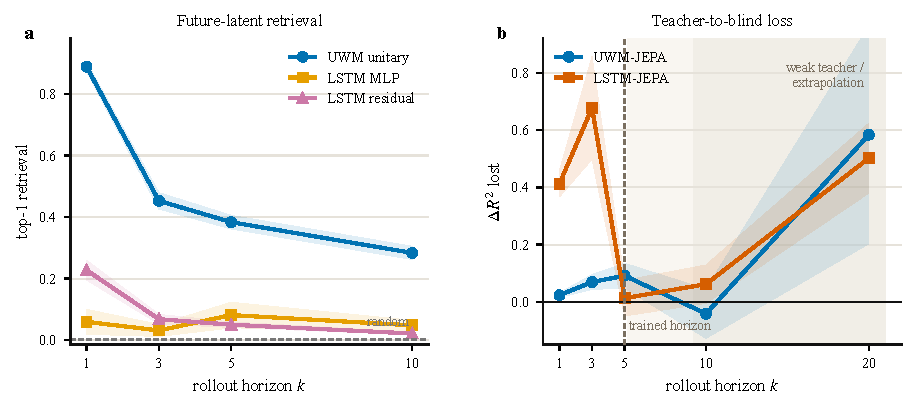
\includegraphics[width=\textwidth]{figures/fig_blind_rollout_evidence.pdf}
\caption{\textbf{Blind-rollout evidence.} \textbf{A}: top-1 retrieval
accuracy for predicted future latents, comparing the UWM unitary
predictor to LSTM-JEPA encoders with plain and residual MLP predictors.
\textbf{B}: information lost under blind rollout, measured as
$\Delta R^2=R^2_{\mathrm{teacher}}-R^2_{\mathrm{blind}}$ for frozen
probes. Lower is better. The dashed vertical line marks the trained
horizon ($k=5$); horizons beyond it are extrapolations, not monotone
information-theoretic forgetting curves. The shaded region marks the
high-variance weak-teacher regime ($k\ge 10$). Together the two panels
show that the context-probe tie in \cref{fig:heldout} does not translate
into matched predictor behaviour.}
\label{fig:blind-rollout}
\end{figure*}

\begin{table*}[t]
\centering
\footnotesize
\setlength{\tabcolsep}{6pt}
\caption{\textbf{Blind-rollout information loss.}
$\Delta R^2=R^2_{\mathrm{teacher}}-R^2_{\mathrm{blind}}$, mean $\pm$
std over three seeds. Lower is better; the headline comparison is
$k=1,3$, before the trained horizon.}
\label{tab:retention}
\begin{tabular}{@{}lccccc@{}}
\toprule
Model & $k{=}1$ & $k{=}3$ & $k{=}5$ & $k{=}10$ & $k{=}20$ \\
\midrule
UWM  & $\mathbf{0.023\pm0.008}$ & $\mathbf{0.069\pm0.026}$ & $0.091\pm0.044$ & $-0.042\pm0.086$ & $0.584\pm0.381$ \\
LSTM & $0.413\pm0.046$ & $0.678\pm0.179$ & $\mathbf{0.013\pm0.062}$ & $0.062\pm0.067$ & $0.502\pm0.122$ \\
\bottomrule
\end{tabular}
\end{table*}

\paragraph{Reading}
UWM-JEPA shows strong short-horizon retention at
$k{=}1$ and $k{=}3$, remains competitive at the trained horizon
$k{=}5$, and degrades by long horizons (\cref{fig:blind-rollout},
panel B; \cref{tab:retention}). Concretely, UWM's $\Delta R^2$ is
$0.023$ at $k{=}1$, $0.069$ at $k{=}3$, and $0.091$ at $k{=}5$: blind
rollout loses less than ten points of $R^2$ relative to what the
target encoder extracts from the true observation at the same horizon.
The matched LSTM-JEPA trained on the same
objective~\cite{hochreiter1997long} has much larger $\Delta R^2$ at
$k{=}1$ and $k{=}3$ ($0.413$ and $0.678$), indicating that its
intermediate blind states are poorly aligned with the target
representation. The LSTM-JEPA re-aligns at $k{=}5$, which is exactly
the horizon used during training; this non-monotonicity is a property
of the learned predictor and probe geometry rather than a physically
monotone information curve. At $k{=}10$ the UWM mean $\Delta R^2$ is
slightly negative, within the reported seed variation, and by $k{=}20$
both models have weak teacher probes and negative blind fits. The
ratio $R^2_{\text{blind}}/R^2_{\text{teacher}}$ is therefore not
reported at $k{=}20$, since dividing two noisy numbers near zero
provides no additional signal.

Short-horizon UWM-JEPA preserves target-nearness better than the
parameter-matched LSTM-JEPA, tracks it at mid horizons, and loses the
signal at long horizons that no tested predictor handles reliably. The
retrieval panel reinforces the same separation: the UWM predictor
improves future-latent retrieval while the LSTM-JEPA models with plain
and residual MLP predictors remain well below it. The pattern is
consistent with the theorem, which constrains only the joint state,
but does not follow from it.
